\section{Gitterdynamik} \label{kap:4}
Physikalische Eigenschaften von FK bestimmt durch:
\begin{itemize}
	\item Bewegung der Atome aus Gleichgewichtslage
	(Schallwellen, spezifische Wärme, Wärmeleitfähigkeit, thermische Ausdehnung etc.)
	\item Bewegung (fast freier) Elektronen (elektronische Eigenschaften)
\end{itemize}
Beide Phänomene sind nicht unabhängig. Hier: Born-Oppenheimer-Näherung (adiabatische Näherung):
\begin{itemize}
	\item Atomrümpfe bewegen aufgrund höherer Masse langsamer als Valenzelektronen.
	\item Verschiebung eines Atomrumpfs $\rightarrow$ 'instantane' Anpassung der Elektronenverteilung.
	Dabei steigt Gesamtenergie des Elektronensystems, die Elektronen bleiben aber im Grundzustand (adiabatischer Prozess)
	\item Atome zurück in GG-Lage. Elektronensystem folgt und kehrt zur ursprünglichen Gesamtenergie zurück.
	\item Alles in Allem: Bewegung der Atomrümpfe $\rightarrow$ Energieänderung des Elektronensystems. 
	$\rightarrow$ Potentialänderung der Atome (\textbf{Gitterdynamik}).
	Elektronen bleiben dabei im Grundzustand, und sind unabhängig von der Bewegung der Atome $\rightarrow$ Beschreibung im
	ursprünglichem periodischen Potential. (\textbf{Elektronensystem} entkoppelt von Gitterdynamik)
\end{itemize}


\subsection{Potential in harmonischer Näherung}		\label{kap:4_1} 
Form des Potentials bestimmt durch Elektronensystem (kompliziert). \\
\textbf{Hier}: Qualitative Betrachtung: \\
Gesamtenergie des Kristalls $\Phi\left( \textbf{r}_{\textbf{n},\alpha} \right)$ hängt von Position 
der Atomrümpfe ($\textbf{n} = (n_1,n_2,n_3)$ Elementarzelle, $\alpha$ Basisposition). Auslenkung aus GG-Position 
$\textbf{r}_{\textbf{n},\alpha}$ sei $\textbf{u}_{\textbf{n},\alpha}$. \\
Taylorentwicklung: \\
% \begin{align}
% 	\Phi\left( \textbf{r}_{\textbf{n},\alpha,i} + \textbf{u}_{\textbf{n},\alpha,i}\right) = \Phi\left( \textbf{r}_{\textbf{n},\alpha,i} \right)
% 	 + \sum_{\textbf{n},\alpha,i} \frac{\partial \Phi}{\partial \textbf{r}_{\textbf{n},\alpha,i}}\vert_{\textbf{u}_{\textbf{n},\alpha,i} = 0\right)}
% 	 + \frac{1}{2} \sum_{\textbf{n},\alpha,i,\textbf{m},\beta,j} \frac{\partial^2 \Phi}{\partial \textbf{r}_{\textbf{n},\alpha,i} \partial \textbf{r}_{\textbf{m},\beta,j}}
% 	 \vert_{\textbf{u}_{\textbf{n},\alpha,i} = 0, \textbf{u}_{\textbf{m},\beta,j} = 0} \textbf{u}_{\textbf{n},\alpha,i} \textbf{u}_{\textbf{m},\beta,j}
% \end{align}

%TODO: Hier fehlt noch was

Atomrümpfe bewegen sich näherungsweise in harmonischem Potential.\\
Weitere Vereinfachungen:
\begin{itemize}
	\item[(i)] Wechselwirkung nur zwischen nächsten Nachbarn.
	(i.d.R. keine langreichweitige WW)
	\item[(ii)] Betrachtung einer 1D Kette von Atomen. (Modell der 1D Kette beschreibt Gitterdynamik eines 3D Kristalls gut)\\
	Ausbreitung einer ebenen Welle in Hochsymmetrierichtung:\\
	Aus Symmetriegründen kompensieren sich Kräfte, die nicht längs der Ausbreitungsrichtung wirken. Es treten entweder longitudinale oder transversale Moden (in Hochsymmetrierichtungen).\\
	\begin{itemize}
		\item[$\rightarrow$] Damit ist 3D Problem auf 1D Modell in Richtung des Wellenvektors zurückgeführt, da Netzebenen $\bot$  Wellenvektor die gleiche Bewegung.
		\item[$\rightarrow$] 1D Bewegungsgleichung mit effektiven Kräften, die Bewegung der gesamten Netzebene beschreiben.
	\end{itemize}
\end{itemize}



\subsection{Modell der linearen Kette} \label{kap:4_2}
\begin{itemize}
	\item[(a)] \textbf{Lineare Kette mit 1-atomiger Basis:}\\
	\begin{figure}[H]
		\centering
		\includegraphics[width=0.8\textwidth]{figures/4_2linKette}
		\caption{}
		\label{}
	\end{figure}
	Rückstellkraft auf s-tes Atom: $F_s = c [(u_{s+1} - u_s) - (u_s - u_{s-1})]$
	Bewegungsgleichung
	\begin{align*}
		m \cdot\frac{\mathrm{d}^2 u_s}{\mathrm{d}t^2} &= c [(u_{s+1} - u_s) - (u_s - u_{s-1})]\\
		\text{Ansatz:} \qquad u_s &= U_0 \cdot e^{-i(\omega t + q s a)}\\
		\Rightarrow \qquad \qquad -\omega^2 \cdot m &= c [e^{-iqa} -1-1+e^{+iqa}]\\
		\omega^2 &= \frac{2 c}{m} [1 - \frac{1}{2} (e^{iqa} +e^{-iqa}]\\
		&= \frac{2 c}{m} (1- \cos(qa))\\
		&= \frac{4 c}{m} \sin^2\left(\frac{qa}{2}\right)
	\end{align*}
	$\Rightarrow$ Dispersionsrelation der linearen Kette: $\omega = 2 \cdot \sqrt{\frac{c}{m}}\left|\sin\left(\frac{qa}{2}\right)\right|$ \\
	\begin{figure}[H]
		\centering
		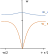
\includegraphics[width=0.4\textwidth]{figures/4_2disp}
		\caption{}
		\label{fig:4_2disrel}
	\end{figure}
	\textbf{Diskussion}: \\
	\begin{itemize}
		\item[(i)] Beschränkung des Wellenvektors auf die 1. Brillouin-Zone: \\
			Phasenunterschied 2er benachbarter Atome: $u_{s+1} / u_{s} = e^{iqa} = e^{i\varphi}$ ist maximal $2\pi$. 
			\begin{itemize}
				\item[$\rightarrow$] Betrachtung des Bereichs $-\pi < qa \le + \pi$  bzw.  $-\pi/a < q \le +\pi/a $ (1.BZ)
				\item[$\rightarrow$] Wellenvektor $q'$ außerhalb 1. BZ: Rücktransformation durch Addition eines geeigneten Gittervektors G
				\begin{align*}
					G = \frac{2 \pi}{a} \cdot p \quad (p \in \mathbb{Z})\text{, also} \quad q' = q + \frac{2 \pi}{a} \cdot p
				\end{align*}
				Begründung: $\frac{u_{s+1}}{u_{s}} = e^{iq'a} = e^{iqa}\cdot e^{i2\pi p} = e^{iqa}$
				\item[$\rightarrow$] Bei Rücktransformation in die 1. BZ kann Wellenvektor das Vorzeichen wechseln. Das entspricht einem VZ-Wechsel der Phasengeschwindigkeit $v_P = \omega / q$. Die Gruppengeschwindigkeit $v_G = \partial\omega / \partial q$ bleibt gleich ($\rightsquigarrow$ Energietransport der Welle).
			\end{itemize}
		\item[(ii)] \textbf{Grenzfälle:} \\
			\begin{itemize}
				\item[(I)] \textbf{Langwelliger Grenzfall:}\\
				$q \rightarrow 0$ bzw. $\lambda = 2 \pi / q \rightarrow \infty$
				\begin{align*}
					\omega \approx 2 \cdot \sqrt{\frac{c}{m}} \cdot \left| \frac{qa}{2} \right| \sim \left| q \right| 
				\end{align*}
				\begin{itemize}
					\item lineare Dispersion
					\item $v_p = \pm \sqrt{\frac{c}{m}}\cdot a $
					\item $v_G = \pm \sqrt{\frac{c}{m}} \cdot a $
				\end{itemize}
				\item[(II)] \textbf{Kurzwelliger Grenzfall:}\\
				$q \rightarrow \pm \pi / a$ bzw. $\lambda = 2 \pi / q \rightarrow 2a$
				\begin{align*}
					\omega \approx 2 \cdot \sqrt{\frac{c}{m}} \left(1-\frac{1}{2} \left( \frac{qa}{2} \right)^2\right) \approx 2 \cdot \sqrt{\frac{c}{m}}
				\end{align*}
				\begin{itemize}
					\item Dispersion $\approx$ konstant
					\item $v_p = \omega / q $, $V_G = \partial \omega / \partial q \to 0$ d.h \textbf{stehende Welle}
					\item relative Phasenlage: $u_{s+1} / u_s = e^{iqa} \quad \rightarrow \quad e^{\pm \pi} = -1$\\
					d.h. benachbarte Atome schwingen für $q \rightarrow \pm \pi / a$ gegenphasig. (stehende Welle mit $\lambda = 2a$)\\
					$\rightsquigarrow$ Auftreten der stehenden Welle kann als konstruktive Interferenz der einlaufenden Welle mit $ q = \pi / a $ und der gebeugten Welle verstanden werden: $ 2 \cdot a \cdot \sin(\theta) = n \cdot \lambda $ (für $n=1$, $\lambda = 2a$) \\
					$2 \cdot a \cdot \sin(\theta) = 2 \cdot a $, also $\theta = \ang{90}$ oder Streuwinkel $\ang{180}$.
					\begin{figure}[H]
						\centering
						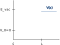
\includegraphics[width=0.4\textwidth]{figures/4_2winkel}
						\caption{}
						\label{fig:4_2winkel}
					\end{figure}
				\end{itemize} 
			\end{itemize}
	\end{itemize}
	\item[(b)] \textbf{Lineare Kette mit 2-atomiger Basis:} \\
		Mit Federkonstante $c$ und Massen $m_A$, $m_B$.
		\begin{figure}[H]
			\centering
			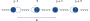
\includegraphics[width=0.8\textwidth]{figures/4_2Kette2}
			\caption{}
			\label{fig:4_2kette2}
		\end{figure} 
		Rückstellkraft:
		\begin{align*}
			F_{A,S} &= c \left[(v_s - u_s) - (u_s - v_{s-1})\right] \\
			F_{B,S} &= c \left[(u_{s+1} - v_s) - (v_s - u_{s})\right] 
		\end{align*}
		Bewegungsgleichungen:
		\begin{align*}
			m_A \cdot \frac{\mathrm{d}^2u_s}{\mathrm{d}t^2} &= c \cdot (v_s + v_{s-1} - 2 u_s) \\
			m_B \cdot \frac{\mathrm{d}^2v_s}{\mathrm{d}t^2} &= c \cdot (u_{s+1} + u_s - 2 v_s)
		\end{align*}
		Ansatz:
		\begin{align*}
			u_s &= U e^{-i(\omega t - q s a)} \\
			v_s &= V e^{-i(\omega t - q s a)}
		\end{align*}
		Ansatz einsetzen, Gleichungssystem lösen (Koeffizientendeterminante = 0):\\
		$\Rightarrow$ Dispersionsrelation:
		\begin{align*}
			\omega_{a,0}^2 = c \left( \frac{1}{m_A} + \frac{1}{m_A} \right) \mp c \sqrt{\left( \frac{1}{m_A} + \frac{1}{m_A} \right)^2 - \frac{4}{m_A m_B} \cdot \sin^2 \left(\frac{qa}{2}\right)}
		\end{align*}
		Maximum: $\tilde{\omega} = \omega_{max} = \sqrt{2c \left( \frac{1}{m_A} + \frac{1}{m_A} \right)} = \sqrt{\frac{2c}{\mu}}$
		\begin{figure}[H]
			\centering
			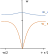
\includegraphics[width=0.4\textwidth]{figures/4_2disp}
			\caption{}
			\label{fig:4_2disp}
		\end{figure}
	\textbf{Diskussion:}\\
	\begin{itemize}
		\item[(A)] \textbf{Zweig $\omega_a$:}\\
		Wie lineare Kette mit 1-atomiger Basis ($m_A = m_B = m$ und $a \rightarrow 2a$)
		\begin{itemize}
			\item[(i)] Langwelliger Grenzfall: $q \rightarrow 0$ ($\lambda \rightarrow \infty$)
			\begin{itemize}
				\item lineare Dispersion
				\item relative Phasenlage benachbarter Atome: $\frac{u}{v} \approx \frac{2c}{2c-\omega_a^2 m_A} \approx 1$ (für $q \rightarrow 0$)\\
				d.h. benachbarte Atome schwingen $\approx$ gleichphasig mit fast gleicher Amplitude.
				% \begin{figure}[H]
				% 	\centering
				% 	\includegraphics[width=0.8\textwidth]{figures/4_2transWelle}
				% 	\caption{Visualisierung: Transversalwelle}
				% 	\label{fig:4_2transWelle}
				% \end{figure}
				$\Rightarrow$ im langwelligen Grenzfall verhalten sich die Gitterwellen wie Schallwellen: \textbf{akustischer Zweig} $\omega_a$.
			\end{itemize}
			\item[(ii)] Kurzwelliger Grenzfall: $q \rightarrow \pm \frac{\pi}{a}$ ($\lambda \rightarrow 2a$): $\omega_a^2 \rightarrow \frac{2c}{m_B}$ ($m_a < m_B$)
			\begin{itemize}
				\item konstante Dispersion
				\item relative Phasenlage $\frac{u}{v} = 0$\\
				d.h. das leichtere Untergitter A ist in Ruhe, das schwerere B schwingt. Benachbarte Atome B schwingen gegenphasig (vgl. (a)) %TODO ref?
			\end{itemize}
		\end{itemize}
		\item[(B)] \textbf{Zweig $\omega_0$:}
		\begin{itemize}
			\item[(i)] $q \rightarrow 0$ ($\lambda \rightarrow \infty$): $\omega_0^2 \approx 2c \left(\frac{1}{m_A} + \frac{1}{m_B}\right) = \frac{2c}{\mu} = \tilde{\omega}^2$
			\begin{itemize}
				\item konstante Dispersion
				\item $\frac{u}{v} \approx - \frac{m_B}{m_A}$
				% \begin{figure}[H]
				% 	\centering
				% 	\includegraphics[width=0.8\textwidth]{figures/4_2VisB}
				% 	\caption{Visualisierung (wie in (A))}
				% 	\label{fig:4_2VisB}
				% \end{figure} 
				d.h.gegenphasige Schwingung.\\
				Interpretation: Sind A, B Ionen mit unterschiedlichen Ladungen, entsteht ein oszillierendes elektrisches Dipolmoment. Damit koppeln Gitterschwingungen an elektromagnetischen Wellen (Infrarotbereich): \textbf{optischer Zweig} $\omega_0$.
			\end{itemize}
			\item[(ii)]  $q \rightarrow \pm \frac{\pi}{a}$ ($\lambda \rightarrow 2a$): $\omega_0^2 \rightarrow \frac{2c}{m_A}$ ($m_a < m_B$),\\
			d.h. für $m_A \neq m_B$ tritt Frequenzlücke auf, in der keine Gitterschwingungen existieren. Das bedeutet Anregung ist $\omega$ im Bereich der Lücke klingen exponentiell ab.
			\begin{align*}
				-\frac{V}{U}\approx \frac{C(1+e^{\pm i\pi})}{2C-\omega_0^2m_B} = 0
			\end{align*}
			,d.h schwereres Untergitter B in Ruhe, A schwingt. Benachbarte Atome im A-Gitter schwingen gegenphasig.
			\item[(iii)] Verallgemeinerung auf reale Kristalle:\\
			Betrachte Ausbreitung in Symmetrierichtung in 3D-Kristall.\\
			Es treten longitudinale (L) oder transversale (T) Schwingungen auf.
		\end{itemize} 
		1-atomige Basis: 1L, 2T (senkrecht aufeinander, falls isotrop, entartet)\\
		\begin{itemize}
			\item[p-atomige Basis:]
			\begin{itemize}
				\item 3p Zweige
				\item 3 akustische (1L. 2T wie oben)
				\item 3p-3 optische ( (1p-1)L,  (2p-2)T )
			\end{itemize} 
		\end{itemize}
		z.B. 2-atomige Basis: 6 Zweige, 3 ak. (\textbf{1L}, 2T), 3 opt. (\textbf{1L}, 2T)
		% \begin{figure}[H]
		% 	\centering
		% 	\includegraphics[width=0.8\textwidth]{figures/4_2VisB.pdf}
		% 	\caption{zwischen -pi/a bis pi/a amplituden manche bei 0 min. manche max}
		% 	\label{fig:4_2VisC}
		% \end{figure}
	\end{itemize}
\end{itemize}




\subsection{Streuung an Kristallen mit zeitlich veränderlichem Gitter} \label{kap:4_3}
 Aus Kap: \ref{kap:3_1} Streuamplitude,
\begin{align*}
	A_B(\Delta \textbf{k})= \underbrace{\frac{A_0}{R^i}e^{i(k'R+k'R')}}_{=: \tilde{\tilde{A}}} e^{i\omega_0t} \underbrace{\int \rho(\textbf{r})e^{-i\Delta kr} dr}_{\text{vgl. kap \ref{kap:3_3}}}
\end{align*}
\begin{itemize}
	\item[\textbf{Ann:}] Kristall mit 1-atomiger Basis (z.B. Neutronenstreuung bisher)
	\item[\textbf{Jetzt:}] $\textbf{r} = \underbrace{\textbf{R}_n}_{\text{GG-Pos. des n-ten Atoms}} + \textbf{u}_n(t)$\\
	Zeitabhängige Auslenkung des n-ten Atoms um GG-Lage.
\end{itemize}
\begin{align*}
	A_B(t) &= \tilde{\tilde{A}} e^{-i\omega_0 t} \sum_n \int \rho(\textbf{r}) e^{-i\Delta \textbf{k} \textbf{R}_n } e^{-i\Delta \textbf{k} \textbf{u}_n(t)} \mathrm{d}^3r\\
	&= \tilde{\tilde{A}} e^{-i\omega_0 t} \sum_n \rho_n e^{-i\Delta \textbf{k} \textbf{R}_n } e^{-i\Delta \textbf{k} \textbf{u}_n(t)} \text{ für punktförmigen Streuer}
\end{align*}
Auslenkung der Gitterschwingung klein gegenüber a, d.h.$\Delta \textbf{k} \textbf{u}_n(t) \ll 1$, damit
\begin{align*}
	A_B(t) \approx \tilde{\tilde{A}} e^{-i\omega_0 t} \sum_n \rho_n e^{-i\Delta \textbf{k} \textbf{R}_n } \left(  1 -i\Delta \textbf{k} \textbf{u}_n(t) - \frac{1}{2}(\Delta \textbf{k} \textbf{u}_n(t))\right)
\end{align*}
Innere Entwicklung:
\begin{align*}
	A_B(t) \approx \tilde{\tilde{A}} e^{-i\omega_0 t} \sum_n \rho_n e^{-i\Delta \textbf{k} \textbf{R}_n } - \tilde{\tilde{A}} e^{-i\omega_0 t} \sum_n \rho_n i\Delta \textbf{k} \textbf{u}_n(t) e^{-i\Delta \textbf{k} \textbf{R}_n}
\end{align*}
Ansatz: 
\begin{align*}
	\textbf{u}_n(t) = \sum_q \textbf{u}_q \cdot e^{\pm i(\textbf{q} \textbf{R} n - \omega_q t)}
\end{align*}
Überlagerung von ebenen Wellen mit $q > 0$.
\begin{align*}
	\rightarrow \quad A_B(t) \approx \underbrace{\tilde{\tilde{A}} e^{-i\omega_0 t} \sum_n \rho_n e^{-i\Delta \textbf{k} \textbf{R}_n }}_{\begin{matrix}
		\text{Beitrag elastischer Streuung}\\
		\text{vgl. Kap. \ref{kap:3_3}}\\
		\text{Wert } \neq 0 \text{ nur für }\\
		\Delta \textbf{k} = \textbf{G}_{hkl}
	\end{matrix}} - \underbrace{\tilde{\tilde{A}} e^{-i\omega_0 t} \sum_n \rho_n i\Delta \textbf{k} \textbf{u}_q e^{-i(\Delta \textbf{k} \mp \textbf{q}) \textbf{R}_n} e^{-i(\omega_0 \pm \omega_q) t}}_{\begin{matrix}
		\text{Beitrag inelastischer Streuung,} \\
		\text{geänderte Streubedingung:}\\
		\Delta \textbf{k} \mp \textbf{q} = \textbf{G}_{hkl} \text{ (Impulserhaltung)}\\
		\omega = \omega_0 \pm \omega_q \text{ (Energieerhaltung)}
	\end{matrix}}
\end{align*}

\subsection*{Inelastische Streuung eines Teilchens: Absorption eines Phonons}

\begin{align*}
	\hbar \omega &= \hbar \omega_0 \pm \hbar \omega_q\\
	\hbar \textbf{k'} &= \hbar \textbf{k} \pm \hbar \textbf{q} + \hbar \textbf{G}_{hkl}
\end{align*}

\subsection{Quantisierung von Gitterschwingungen}  \label{kap:4_4}

\begin{itemize}
	\item[bisher:] klassische Betrachtung, lineare Kette (hier: 1-atomige Basis) aus N Atomen.
	\item Jedes Atom: 3 Schwingungsmoden, insgesamt: 3N Normalmoden der kollektiven Bewegung der Atome
	\item Periodische Randbedingungen: $u_s \overset{!}{=} u_{s+N}$
	\begin{align*}
		\text{d.h.} \qquad u_0 e^{-i(\omega t + q \cdot s \cdot a)} &\overset{!}{=} u_0 e^{-i(\omega t + q \cdot s \cdot a + q \cdot N \cdot a)}\\
		\Leftrightarrow \qquad e^{-iqNa} \overset{!}{=} 1 \quad &\Leftrightarrow \quad q \overset{!}{=} \frac{2 \pi}{a} \cdot \frac{p}{N} \quad \text{mit} \quad p \in \mathbb{Z}
	\end{align*}
	für Wellenvektoren in der 1. BZ: $-\frac{N}{2} < p \leq + \frac{N}{2}$
	% \begin{figure}[H]
		% 	\centering
		% 	\includegraphics[width=0.8\textwidth]{figures/4_moden.png}
		% 	\caption{}
		% 	\label{fig:4_moden.png}
	% \end{figure}
	\begin{itemize}
		\item[$\rightarrow$] 3N Lösungen: Schwingungsmoden
	\end{itemize}
	Quantisierung: Jede Mode entspricht einem QM harmonischen Oszillator mit Energie $E_{q,j} = \hbar \omega_j(\textbf{q})(n_{qj} + \frac{1}{2})$ mit Wellenvektor \textbf{q} und $j$ = 1,2,3 Zweig-Index
\end{itemize}
\paragraph{Diskussion:}
\begin{itemize}
	\item[(1)] Bestimmter Schwingungszustand $\omega_j(\textbf{q})$ kann nur diskrete Energiewerte annehmen ($n_{qj} = 0,1,2,\dots$), je nach Besetzungszahl der Normalmode mit \textbf{q} im Zweig j.\\
	d.h. die Energie der Gitterschwingungen ist quantisiert.\\
	Welle-Teilchen-Dualismus: Das Quant der Gitterschwingung wird als \textbf{Phonon} bezeichnet.
	\begin{itemize}
		\item[$\rightarrow$] Gitterschwingung als quantisierte \textbf{Anregung der gesamten Kristalls} ODER
		\item[$\rightarrow$] Gitterschwingung als \textbf{Quasiteilchen} mit\\
		Energie $E_j(\textbf{q}) = \hbar \omega_j(\textbf{q})$\\
		Impuls $\textbf{p} ( \textbf{q}) = \hbar \textbf{q} = \hbar \textbf{q} + \hbar \textbf{G} $ (!Quasi-Impuls (Kristallimpuls)!)\\
		$\rightsquigarrow$ nur bis auf \textbf{G} festgelegt, d.h. Translationsinvarianz nur bzgl. \textbf{G}. (Physikalischer) Impuls des Kristalls
		\begin{align*}
			p &= m \cdot \frac{\mathrm{d}}{\mathrm{d}t} \sum_{\textbf{n} \alpha} u_{\textbf{n} \alpha} = m \cdot \frac{\mathrm{d}}{\mathrm{d}t} \sum_s u_0 e^{-i(\omega t + q  s a)}\\
			&= -i \omega m u_0 e^{-i \omega t} \sum_s e^{-i q s a} = -i \omega m u_0 e^{-i \omega t} \frac{1 - e^{-i q N a}}{1 - e^{-i q a}} \underset{\begin{matrix}
				\uparrow\\ 
				q = \frac{2 \pi}{a} \cdot \frac{p}{N}
			\end{matrix}}{=} 0
		\end{align*}
	\end{itemize}
\end{itemize}


\subsection{Experimentelle Bestimmung von Dispersionsrelationen} \label{kap:4_5}

Phononen (am Rand der 1. BZ):
\begin{align*}
	\lambda &\approx 2a \approx 3.6 \text{\AA}\\
	\nu &\approx 5 \text{THz}\\
	\hbar \omega &\approx 3.3 \cdot 10^{-21} \text{J} \approx 10^{-2} \text{eV}\\
	u &\approx 5 \cdot 10^{-23} \text{m}\\
	n_q &\approx 1.5 \cdot 10^{23} 1/\text{cm}^3 \approx N (\text{bei 300 K})
\end{align*}

\subsection*{Messung von Phononen:}
\begin{itemize}
	\item[(a)] \textbf{Kohärente inelastische Streuung mit Neutronen:}
	\begin{itemize}
		\item thermische Neutronen ($E \approx$ 100 meV)
		\item relative Energieänderung durch Phonon an BZ-Grenze
		\begin{align*}
			\frac{\delta E}{E} = \frac{10^{-2} \text{eV}}{10^{-1} \text{eV}} \approx \frac{1}{10}
		\end{align*}
	\end{itemize}
	\item[(b)] \textbf{Kohärente inelastische Röntgenstreuung}
	\begin{itemize}
		\item Röntgenlicht ($E \approx$ 10 keV) hat deutlich kleineres
		\begin{align*}
			\frac{\delta E}{E} = \frac{10^{-2} \text{eV}}{10^{4} \text{eV}} \approx 10^{-6}
		\end{align*}
		d.h. Dispersion der Phononen ist experimentell schwer aufzulösen.
	\end{itemize}
	\item[(c)] \textbf{Lichtstreuung:}
	\begin{itemize}
		\item sichtbares Licht ($E \sim$ 100 meV) liefert
		\begin{align*}
			\frac{\delta E}{E} = \frac{10^{-2} \text{eV}}{10^{-1} \text{eV}} \approx \frac{1}{10}
		\end{align*}
		gut auflösbar, aber $\lambda \gg a$ (d.h. $k = \frac{2 \pi}{\lambda} \ll \frac{2 \pi}{a}$, also im Zentrum der 1. BZ)\\
		d.h. Phononendispersion, aber nur für $q$ = 0.\\
		Damit Formulierung Impulserhaltung nur in 1. BZ: $\textbf{k'} = \textbf{k} \pm \textbf{q}$
		\begin{itemize}
			\item[(i)] $q$ = 0: Streuung ohne Phononen. Rayleigh-Streuung
			\item[(ii)] $q \neq 0$: Streuung unter Emission/Absorption eines Phonons: Raman (o. Brillouin)-Streuung
		\end{itemize}
	\end{itemize}  
\end{itemize}



\subsection{Spezifische Wärmekapazität des Kristallgitters} \label{kap:4_6}

Definition (Thermodynamik):
\begin{align*}
	C_p = \left( \frac{\partial U}{\partial T} \right)_p \quad , \quad C_V = \left( \frac{\partial U}{\partial T} \right)_V
\end{align*}
$U$: Innere Energie, $p$: Druck, $V$: Volumen mit $C_p - C_V = \frac{9 \alpha^2}{\kappa} \cdot V \cdot T$ ($\alpha$: lineare thermische Ausdehnung, $\kappa$: Kompressibilität)\\
In Festkörpern ist $\alpha$ sehr klein, so dass $\underset{\begin{matrix}
	\uparrow\\
	Messung
\end{matrix}}{C_p} \approx \underset{\begin{matrix}
	\uparrow\\
	Theorie
\end{matrix}}{C_V}$\\
\begin{itemize}
	\item[Hier:] Beitrag von Gitterschwingungen zu $C_V$ $\rightarrow$ dielektrischer FK
	\item[Später:] Beitrag von Leitungselektronen zu $C_V$ $\rightarrow$ metallische FK 
\end{itemize}

\begin{itemize}
	\item[(a)] \textbf{Zustandsdichte der Phononen}
	\begin{itemize}
		\item Kristall ist (idealisiert) unendlich groß (Translationssymmetrie)\\
		$\rightarrow$ Gitterschwingungen: ebene Wellen, kontinuierliches \textbf{q}
		\item realer Kristall: $N$ Elementarzellen mit $p$ Atomen, also $p \cdot N$ Atome\\
		$\rightsquigarrow$ schwierig
		\item Lösung: periodische Randbedingungen: Für Auslenkungen 
		\begin{align*}
			&\qquad \textbf{u}(\textbf{r},t) = \textbf{U}_{\textbf{q}} e^{-i(\omega_q t - \textbf{q} \textbf{r})}\\
			&\text{mit} \qquad \textbf{u}(x,y,z,t) \overset{!}{=} \textbf{u}(x+L,y,z,t) \overset{!}{=} \textbf{u}(x,y+L,z,t) \overset{!}{=} \textbf{u}(x,y,z+L,t)\\
			&\Rightarrow \qquad e^{i q_x L} = e^{i q_y L} = e^{i q_z L} \overset{\begin{matrix}
				\text{für Kantenlänge $L$}\\
				!
			\end{matrix}}{=} 1\\
			&\Rightarrow\qquad q_i = \frac{2\pi}{L} \cdot m_i \quad \text{für} \quad i=1,2,3\qquad \text{mit}\quad-\frac{\sqrt[3]{N}}{2}<m_i \leq +\frac{\sqrt[3]{N}}{2}
		\end{align*}
		d.h. $q$ hat $(\sqrt[3]{N})^3 = N$ diskrete Werte für jeden Zweig, also insgesamt $3 \cdot p \cdot N$ Wellenvektoren (=Normalmoden)\\
		Es ist mit $\textbf{b}_i = \frac{2 \pi}{V_0} (\textbf{a}_j \times \textbf{a}_k)$:
		\begin{align*}
			\textbf{q} = \sum_{j = 1,2,3} \frac{m_i \cdot \textbf{b}_i}{\sqrt[3]{N}}
		\end{align*}
	\end{itemize} 


\textbf{Zustandsdichte im k-Raum}: Zahl der möglichen Zustände im reziproken Raum pro Volumen alle erlaubten q liegen in 1.BZ, damit
\begin{align*}
	D(q) = \frac{(\sqrt[3]{N})^3}{(2\pi)^3/V_0} = \frac{N \cdot V_0}{(2\pi)^3} = \frac{V}{(2\pi)^3}
\end{align*}
\textbf{NB}: analog für 2D und 1D:
\begin{align*}
	D^{2d}(q) &= \frac{(\sqrt{N})^2}{(2\pi)^2/A_0} = \frac{A}{(2\pi)^2} \\
	D^{1d}(q) &= \frac{N}{(2\pi)^2/L_0} = \frac{L}{(2\pi)^2}
\end{align*}

\textbf{Zustandsdichte im Frequenz-Raum}: Zahl der Zustände im Frequenzraum pro Volumen.\\
Bestimmung aud Dispersionsrelation:
% \begin{figure}[]
% 	\centering
% 	\includegraphics{figures/4_2gitter.pdf}
% 	\caption{Zustaende, dieser Frequenz zwischen $w(q)=\text{const}$} und $\omega+\mathrm(d)\omega=\text{const}$ liegen}
% 	\label{}
% \end{figure}

Integration (statt Summen, wegen grossen Zahlen von Atomen): $q(\omega+\mathrm{d}\omega)$

\begin{align*}
	\int_{\omega(q)=const}^{\omega+\mathrm{d}\omega = const} D(\omega)\mathrm{d}\omega = \int_{q(\omega)}^{q(\omega+\mathrm{d}\omega)} D(q)\mathrm{d}^3q
	= \frac{V}{(2\pi)^3}\int\mathrm{d}S_\omega\mathrm{d}q_\bot 
\end{align*}
wobei $ \mathrm{d}^3q = \mathrm{d}S_\omega \cdot \mathrm{d}q_\bot $ erstetzt wurde mit $\mathrm{d}S_\omega$ Flächenelement und $\mathrm{d}q_\bot$ Flächennormale.
Mit $v_g = \left|\frac{\mathrm{d}\omega}{\mathrm{d}q}\right| = \left|\text{grad}_q\omega\right| = \frac{\mathrm{d}\omega}{\mathrm{d}q_\bot} $ folgt
\begin{align}
	= \frac{V}{(2\pi)^3} \mathrm{d}\omega \int_{\omega = const} \frac{\mathrm{d}S_\omega}{\left|grad_q\omega\right|}
\end{align}
Damit:
\begin{align*}
	D(\omega) \mathrm{d} \omega \tilde{=} \int_{\omega(q)=const}^{\omega+\mathrm{d}\omega = const} D(\omega)\mathrm{d}\omega = \frac{V}{(2\pi)^3} \int \frac{\mathrm{d}S_{\omega}}{(\text{grad}_{q} \omega)} \mathrm{d}\omega
\end{align*}

$\rightarrow$ $D(\omega)$ ist hoch, wenn die Dispersionskurve flach ist.\\
Extremfall: $D(\omega)$ divergiert für $v_g = 0$ (van-Hore Singularitäten)\\
$\rightarrow$ für isotrope FK: Fläche konstanter Frequenz im rez. Raum $S_{\omega}$ ist Kugel mit Radius $|\textbf{q}|$:
\begin{align}
	\Rightarrow D(\omega) = \frac{V}{(2\pi)^3} \cdot \frac{4\pi q^2}{v_g} = \frac{V}{2\pi^2} \cdot \frac{q^2}{v_g}
\end{align}
\item[(b)] \textbf{Debye-Modell:}\\
\textbf{Annahmen:} \begin{itemize}
	\item[(1)] isotroper Festkörper
	\item[(2)] 1-atomige Basis (nur akustische Moden)
	\item[(3)] lineare Dispersion $\omega = c \cdot q$ (vgl. langwelliger Grenzfall) d.h. FK als elastisches Kontinuum mit Schallgeschwindigkeit $c$
	$$\Rightarrow D(\omega) = \frac{V}{2 \pi} \cdot \frac{\omega^2}{c^3}$$
	Gesamtzahl der Zustände: $\int_0^\infty D(\omega)\mathrm{d}\omega$ divergiert, Widerspruch zur Zahl von Phononenmoden pro Zweig. \\
	$\rightsquigarrow$ Trick: Abschneidefrequenz $\omega_{max}$\\
	\begin{align*}
		\int_0^{\omega_{max}} D(\omega)\mathrm{d}\omega &= \int_0^{\omega_{max}} \frac{V}{2 \pi^2} \frac{\omega^2}{c^3} = \frac{V}{6 \pi^2} \frac{\omega^3}{c^3} \overset{!}{=} N\\
		\Rightarrow \quad \omega_{max} &= \sqrt[3]{\frac{6 \pi^2 N}{V}} \cdot c
	\end{align*}
	Berücksichtigung aller 3 Zweige: $D(\omega)\mathrm{d}\omega = \frac{V}{2\pi^2} \underbrace{\left(\frac{1}{c_L^3} + \frac{2}{c_T^3}\right)}_{=: \frac{3}{c_D^3}} \omega^2\mathrm{d}\omega$\\
	mit der Debye-Geschwindigkeit $c_D$.

\item[(c)]\textbf{Mittlere thermische Energie eines Phonons:}
	statistische Physik: mittlere thermische Besetzung $<n>_T = \frac{1}{e^{\hbar\omega/k_BT}-1}$ (Bose-Einstein-Verteilungsfunktion)

\item[(d)]\textbf{Spezifische Wärmekapazität im Debye-Modell:}
	Beitrag Gitterschwingung zur inneren Energie
	\begin{align}
		U(T) &= \int_0^{\omega_p} \hbar\omega_{q,j} \cdot D(\omega_{q,j}) \cdot <n_{q,j}(\omega,T)> \mathrm{d}\omega = \frac{9N}{\omega_D^3} \int_0^{\omega_D} \frac{\hbar\omega_{q,j}^3\cdot\mathrm{d}\omega}{e^{\hbar\omega_{q,j}/k_BT}-1} \\
		\Rightarrow \quad C_V &= \left(\frac{\partial U}{\partial T}\right)_V = q N k_B \left(\frac{T}{\Theta}\right)^3 \cdot \int_0^{x_D} \frac{e^x x^4 \mathrm{d}x}{(e^x-1)^2}
	\end{align}
	mit $x = \frac{\hbar\omega_{q,j}}{k_BT}$ und $x_D = x(\omega=\omega_D)$ und $k_B\theta = \hbar\omega_D$.

\end{itemize}

\end{itemize}
